\documentclass[aspectratio=169]{beamer}
\usepackage{lmodern}
\usepackage{amsmath, amssymb, amsfonts, amsthm}
\usepackage{cancel}
\usepackage[output-complex-root=j]{siunitx}
\usepackage[american, nooldvoltagedirection]{circuitikz}
\usepackage{bm}
\usepackage{listings}
\usepackage{graphicx}
\usepackage{hyperref}

\usetheme{Berkeley}
\usefonttheme[onlymath]{serif}
\AtBeginSection[]{
    \begin{frame}
    \vfill
    \centering
    \begin{beamercolorbox}[sep=8pt,center,shadow=false,rounded=false]{title}
        \usebeamerfont{title}\insertsectionhead\par
    \end{beamercolorbox}
    \vfill
    \end{frame}
}

\newcommand{\N}{\mathbb{N}}
\newcommand{\Z}{\mathbb{Z}}
\newcommand{\Q}{\mathbb{Q}}
\newcommand{\R}{\mathbb{R}}
\renewcommand{\C}{\mathbb{C}}
\newcommand{\unit}[1]{\bm{\hat{#1}}}
\newcommand{\iprod}[2]{\left\langle #1, #2 \right\rangle}
\newcommand{\tpose}[1]{\left[#1\right]^{\! \top} \!\!}
\newcommand{\diff}[1]{\frac{d}{d #1}}

\title{EECS 16B CSM}
\author{Bryan Ngo}
\date{2020-09-21}
\institute{Computer Science Mentors}

\begin{document}

\begin{frame}
    \maketitle
\end{frame}

\begin{frame}
    \tableofcontents
\end{frame}

\begin{frame}
    \frametitle{Logistics}

    \begin{itemize}
        \item Quest?
        \item Focus for today?
        \item messenger chat
        \item all slides available at \url{https://github.com/bdngo/16b-csm}
    \end{itemize}
\end{frame}

\section{Differential Equations}

\begin{frame}
    \frametitle{Differential Equations}

    Concept check! \pause

    \begin{equation}
        \diff{t} x(t) = f(x, t)
    \end{equation}
    \begin{itemize}
        \item Focusing on first-order ODEs
        \item Relates the derivative in other terms
        \item \href{https://youtu.be/p_di4Zn4wz4?list=PLZHQObOWTQDNPOjrT6KVlfJuKtYTftqH6}{3Blue1Brown video}
    \end{itemize}
\end{frame}

\begin{frame}
    \frametitle{Exponential Differential Equation}
    \framesubtitle{Homogeneous}

    \begin{equation}
        \diff{t} x(t) = \lambda x(t) \implies x(t) = x_0 e^{\lambda t}
    \end{equation}
\end{frame}

\begin{frame}
    \frametitle{Exponential Differential Equation}
    \framesubtitle{Non-Homogeneous}

    \begin{equation}
        \diff{t} x(t) = \alpha x(t) + \beta
    \end{equation}
\end{frame}

\section{RC Circuits}

\begin{frame}
    \frametitle{Undamped Response}

    \begin{center}
        \begin{circuitikz}\draw
            (0, 2) to[C=\(C\), v=\(V_C\), invert] (0, 0)
            (0, 2) to[short, i=\(I_C\)] (2, 2) to[R=\(R\)] (2, 0) to[short] (0, 0)
        ;\end{circuitikz}
    \end{center} \pause
    
    \begin{align}
        C \diff{t} V_C &= -\frac{V_C}{R} \\
        \diff{t} V_C &= \underbrace{-\frac{1}{RC}}_{\lambda} V_C \\
        \Rightarrow V_C(t) &= V_0 e^{-\frac{1}{RC} t} = V_0 e^{-\frac{1}{\tau} t}
    \end{align}
\end{frame}

\section{Vector Differential Equations}

\begin{frame}
    \frametitle{General Form}

    \begin{equation}
        \diff{t} \bm{x}(t) = \bm{Ax}(t) + \bm{Bu}(t)
    \end{equation}
    \begin{itemize}
        \item if \(\bm{A}\) is diagonal, simply a bunch of exponential differential Equations
        \item if not, we can try to diagonalize
    \end{itemize}
\end{frame}

\section{Change of Basis}

\begin{frame}
    \frametitle{Motivation}

    \begin{itemize}
        \item conversion from one linear coordinate system to another
        \item \href{https://youtu.be/P2LTAUO1TdA?list=PLZHQObOWTQDPD3MizzM2xVFitgF8hE_ab}{Yet another 3Blue1Brown video}
    \end{itemize}
\end{frame}

\begin{frame}
    \frametitle{A Visualization}

    \begin{center}
        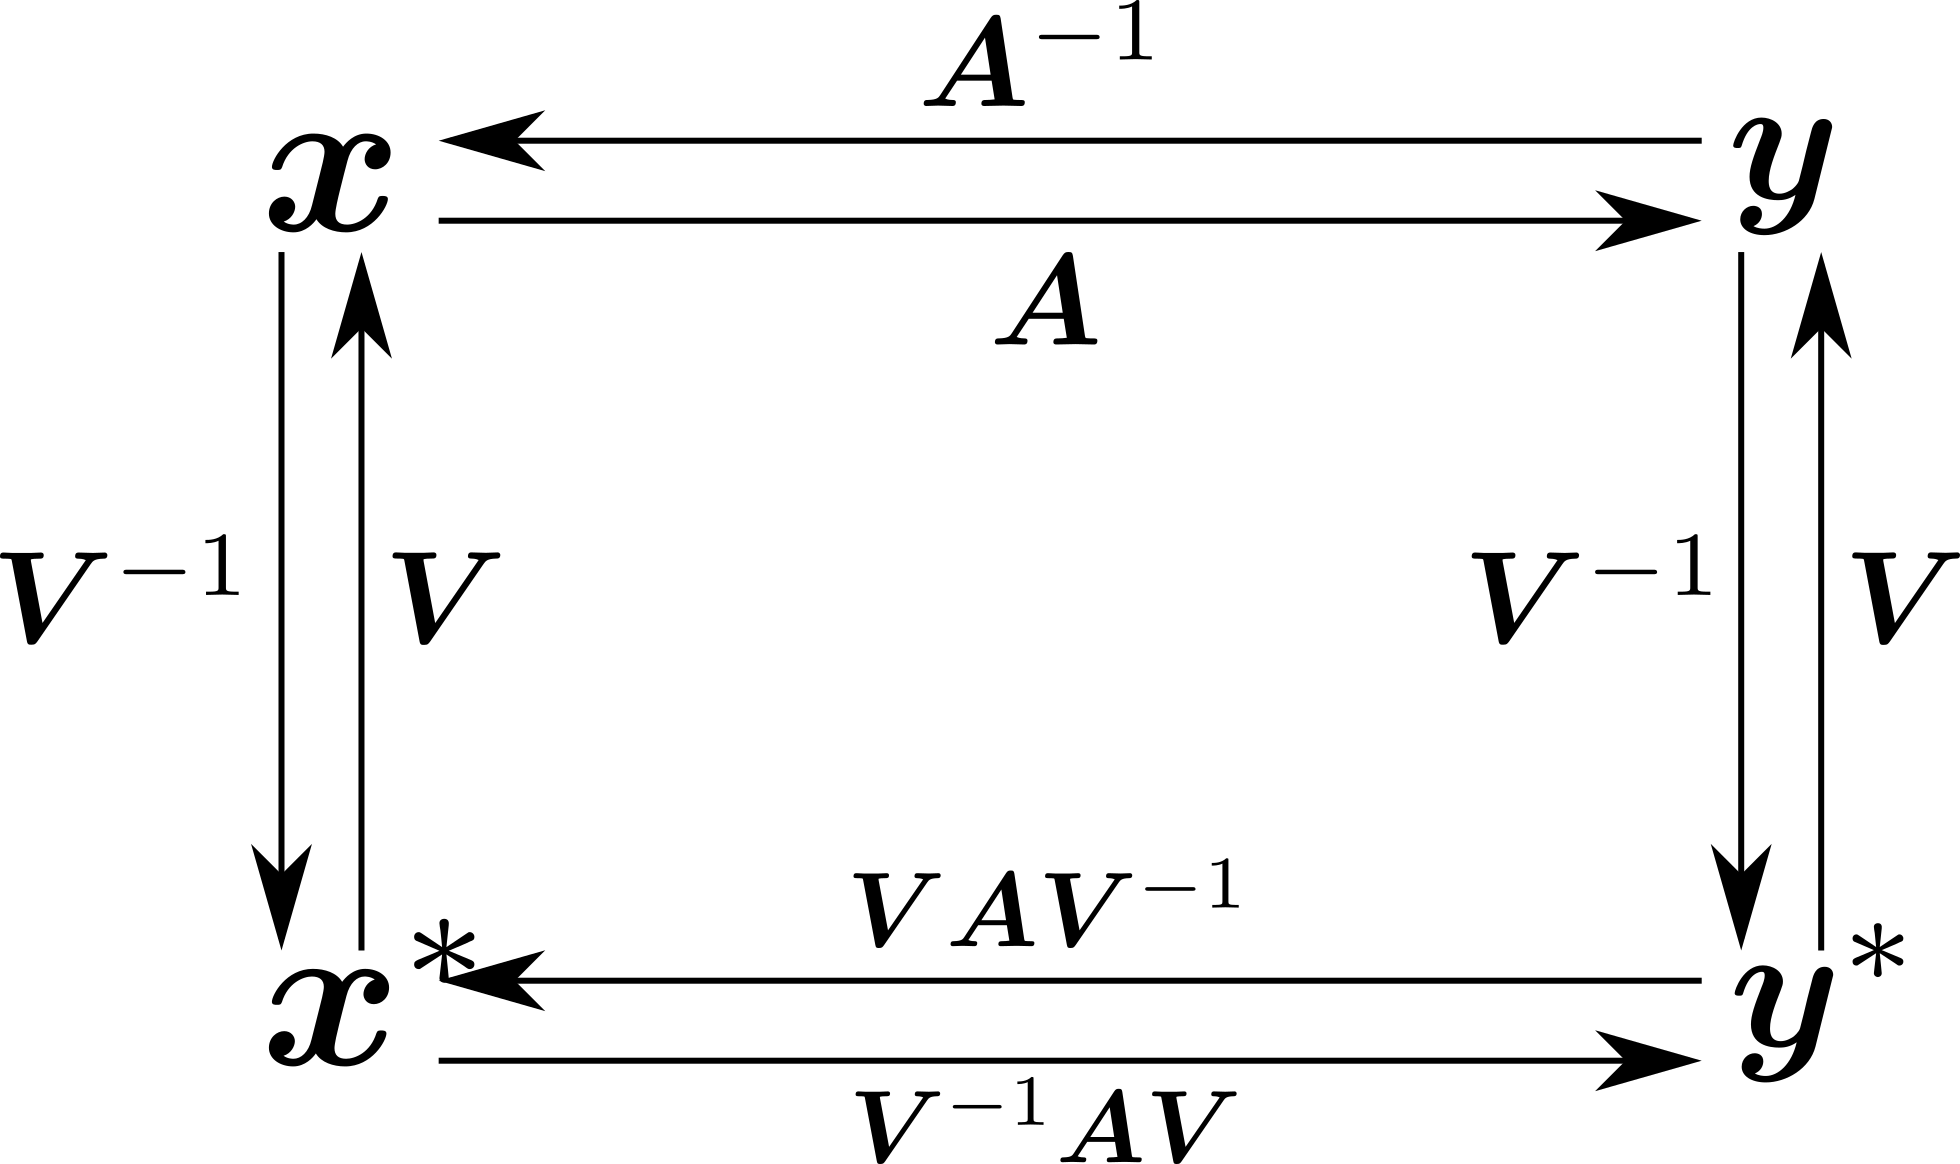
\includegraphics[width=0.8\textwidth]{change-of-basis.png}
    \end{center}
\end{frame}

\begin{frame}
    \frametitle{Diagonalization}

    \begin{itemize}
        \item want the eigenvectors to be the basis for a vector space
        \item makes math \emph{way} easier
    \end{itemize} \pause
    \begin{align}
        \bm{V} &=
        \begin{bmatrix}
            \bm{v}_1 & \bm{v}_2 & \cdots & \bm{v}_n \\
        \end{bmatrix} \\
        \bm{AV} &=
        \begin{bmatrix}
            \lambda_1 \bm{v}_1 & \lambda_2 \bm{v}_2 & \cdots & \lambda_n \bm{v}_n \\
        \end{bmatrix} \\
        &=
        \begin{bmatrix}
            \bm{v}_1 & \bm{v}_2 & \cdots & \bm{v}_n \\
        \end{bmatrix}
        \begin{bmatrix}
            \lambda_1 & 0 & \cdots & 0 \\
            0 & \lambda_2 & \cdots & 0 \\
            \vdots & \vdots & \ddots & \vdots \\
            0 & 0 & \cdots & \lambda_n
        \end{bmatrix} \\
        &= \bm{V \Lambda} \implies \bm{\Lambda} = \bm{V}^{-1} \bm{AV}
    \end{align}
\end{frame}

\begin{frame}
    \frametitle{Diagonalizing DEs}

    \begin{align}
        \diff{t} \bm{x}(t) &= \bm{Ax}(t) + \bm{Bu}(t) \\
        \diff{t} \bm{Vz}(t) &= \bm{AVz}(t) + \bm{Bu}(t) \\
        \Rightarrow \diff{t} \bm{z}(t) &= \bm{V}^{-1} \bm{AVz}(t) + \bm{V}^{-1} \bm{Bu}(t) \\
        &= \bm{\Lambda z}(t) + \bm{V}^{-1} \bm{Bu}(t)
    \end{align}
\end{frame}

\section{Inductors (Preview)}

\begin{frame}
    \frametitle{Basic Properties}

    \begin{center}
        \begin{circuitikz}\draw
            (0, 2) to[L=\(L\), v=\(V_L\), i>^=\(I_L\)] (0, 0)
        ;\end{circuitikz}
    \end{center}
    \begin{equation}
        V_L = L \diff{t} I_L
    \end{equation}
    \begin{itemize}
        \item like a capacitor but for magnetic fields
        \item resists instantaneous change in current \pause
        \item what happens when \(\omega = 0\)? \(\omega = \infty\)?
    \end{itemize}
\end{frame}

\end{document}
